% Created with jtex v.1.0.18
\documentclass{article}
\usepackage{arxiv}

\usepackage[utf8]{inputenc} % allow utf-8 input
\usepackage[T1]{fontenc}    % use 8-bit T1 fonts
\usepackage{hyperref}       % hyperlinks
\usepackage{url}            % simple URL typesetting
\usepackage{datetime}       % show dates in the title block
\usepackage{booktabs}       % professional-quality tables
\usepackage{amsfonts}       % blackboard math symbols
\usepackage{nicefrac}       % compact symbols for 1/2, etc.
\usepackage{microtype}      % microtypography
\usepackage{graphicx}
\usepackage{natbib}
\usepackage{doi}
\usepackage{xcolor}

%%%%%%%%%%%%%%%%%%%%%%%%%%%%%%%%%%%%%%%%%%%%%%%%%%
%%%%%%%%%%%%%%%%%%%%  imports  %%%%%%%%%%%%%%%%%%%
\usepackage{amsmath}
\usepackage{framed}
%%%%%%%%%%%%%%%%%%%%%%%%%%%%%%%%%%%%%%%%%%%%%%%%%%


\hypersetup{colorlinks = true,
linkcolor = purple,
urlcolor  = blue,
citecolor = cyan,
anchorcolor = black}

\title{Reproducibility Standards for Economics}

\newdate{articleDate}{29}{9}{2024}
\date{\displaydate{articleDate}}

\makeatletter
\let\@fnsymbol\@arabic
\makeatother

\author{\href{https://orcid.org/0000-0002-5289-7054}{
\includegraphics[scale=0.06]{orcid.pdf}}\hspace{1mm}Alan Lujan\footnotemark[1]\\
Johns Hopkins University AAP\\Econ-ARK\\\AND
\href{https://orcid.org/0000-0003-3732-9312}{
\includegraphics[scale=0.06]{orcid.pdf}}\hspace{1mm}Chris Carroll\\
Johns Hopkins University\\Econ-ARK\\\AND
Econ-ARK Team\\
}

% Uncomment to override  the `A preprint' in the header
\renewcommand{\headeright}{Project Report}
\renewcommand{\undertitle}{FOSSProF Final Report}
\renewcommand{\shorttitle}{}

%% Add PDF metadata to help others organize their library
%% Once the PDF is generated, you can check the metadata with
%% $ pdfinfo template.pdf
\hypersetup{
pdftitle={\@title},
pdfsubject={},
pdfauthor={\@author},
pdfkeywords={},
addtopdfcreator={Written in Curvenote}
}

\begin{document}
\maketitle
\footnotetext[1]{Correspondence to: alujan@jhu.edu}



\section{Project Overview}

\subsection{Project Summary}

% Briefly describe the project, its objectives, and the open source software it focused on.

The Economics profession needs to catch up to other technical fields in software development, reproducibility practices, and ``exchangeability'' of results.

To that end, \href{https://econ-ark.org}{Econ-ARK} has been working for several years on the \href{https://github.com/econ-ark/REMARK}{REMARK} project, a set of standards and tools for reproducibility for computational modeling in economics. \href{https://econ-ark.org/materials/}{REMARKs} are self-contained and complete projects whose contents should be executable by anyone on any modern computer (local or cloud), so long as the platform has the necessary hardware (generically described). A critical aspect of REMARKs is the emphasis on clear documentation, testing procedures, and standardized metadata to ensure that research outputs are reproducible, understandable, reusable, and securely attributable to their true authors.

The design specs of the REMARK standard have been crafted with the collaboration of the editor of a projected journal that would require all submissions to abide by the REMARK standard.

While we have solved most of the computational challenges (using the blossoming ecosystem of tools including Docker containers, version control, etc.), one piece of the infrastructure needed to complete the specification is still lacking: A robust, reproducible, and portable standard for the production of the text of the paper (or other research product) that can directly integrate reproducible content.

The project sponsored by FossProf allowed us to hire an open-source contractor, \href{https://curvenote.com}{Curvenote}, to fill some crucial gaps in the infrastructure necessary to translate the standard medium of technical writing, $\LaTeX$, to the new world of lightweight, reproducible content. The bulk of the other FossProf funding allowed some JHU PhD students to create new examples of REMARKs that use these tools.

\subsubsection{A brief history of REMARK}

The REMARK project started as a means to enhance the sharing and reproducibility of research that utilized the \href{https://econ-ark.org}{Econ-ARK}'s \href{https://docs.econ-ark.org}{HARK} toolkit. As the development of \href{https://github/econ-ark/HARK}{HARK} was guided mainly by active research, it was essential to expand the codebase and integrate the code with the documentation and drafting of academic manuscripts. In economics, however, the standard practice is to treat the research manuscript and code as entirely separate entities, with the code being used as a tool to generate results that are posted in the manuscript but then relegated to a \texttt{.zip} file attached to the published paper. Because there are no standards for the contents of these zip files, there is no real guarantee that the code can be run by anyone other than the original author(s) on the original computer(s) on which it was developed with the exact software configuration on that computer at the time the final version of the code was zipped. This practice severely limits scholars' ability to reproduce and build upon previous work.

Recognizing the need to integrate scientific software development with the publication of research, \href{https://econ-ark.org}{Econ-ARK} began working on the REMARK standard to make the models and results from the HARK toolkit easy to share. But as the REMARK project grew, it became clear that such a lightweight standard for reproducible computational results could be helpful for the broader Economics community (and perhaps more broadly in the scientific computing community).

\subsection{Target Audience}

% Who are the primary users or beneficiaries of the project? Are there secondary groups that benefit?

The original intended users of REMARKs were students, researchers, and practitioners of economics who would benefit from reproducibility of economic modeling results. However, nothing about the project limits the scope of its use to economics; there is no reason the standard could not be used in any field in which computational results need to be reproducible. As we have worked on the REMARK standard, we have come to realize that there is a broader need for reproducible research practices in many fields where computational results are important to the substantive conclusions of the research.

\subsection{Code Repository}

% Please include links to publicly available code repositories.

This project is a collaboration between the \href{https://econ-ark.org/team}{Econ-ARK team} and \href{https://curvenote.com}{Curvenote}. The \href{https://github.com/econ-ark/REMARK}{REMARK} standard itself can be found at the \href{https://github.com/econ-ark/REMARK}{REMARK GitHub repository}, but much of the code generated during this project has already been integrated into the \href{https://myst-parser.readthedocs.io/en/v0.16.0/}{MyST} project.

\begin{framed}
\textbf{Tip}\\
\begin{itemize}
\item The \href{https://github.com/econ-ark/REMARK}{R[eplications/eproductions] and Explorations Made using ARK} project is publicly available on GitHub.
\item This project led to many contributions to the \href{https://mystmd.org/}{MyST} project, which provides a collection of tools for working with MyST Markdown. MyST is part of \href{https://jupyter.org}{Project Jupyter} and is open source and \href{https://github.com/jupyter-book/mystmd}{publicly available on GitHub}.
\end{itemize}
\end{framed}

\section{Project Activities and Progress}

\subsection{Work Completed}

% Clearly outline the activities undertaken during the grant period. Did you achieve all your planned goals? If not, explain why and what was accomplished instead.

The primary goal of this project was to integrate the \href{https://github.com/jupyter-book/mystmd}{MyST} Markdown tools into the \href{https://github.com/econ-ark/REMARK}{REMARK} project to expand the range of tools available for the standard. To do this, we identified three existing REMARKs that highlighted gaps in the open-source tooling for typesetting and integrating reproducible results directly into a REMARK. Through these examples, we prioritized our contractors, \href{https://curvenote.com}{Curvenote} (who are core MyST developers and members of the steering council), and identified efficient ways to integrate MyST into REMARKs.

We also worked with some Johns Hopkins Economics PhD students to produce REMARKs of their projects, providing feedback on the REMARK standard and showing how the REMARK standard can produce high-quality, reproducible research.

Lastly, we gave a presentation of the REMARK project at the \href{https://comp-econ.com/30th-conference/}{30th International Conference for Computation in Economics and Finance}, where we engaged with many students and researchers interested in open source software for reproducible research and advocated for the adoption of REMARKs as a standard for reproducible research in economics. (The project lead for the REMARK project is the incoming president of the sponsor of the conference, the \href{https://comp-econ.com/}{Society for Computational Economics}.

\subsubsection{Collaboration with Myst/Curvenote}

Throughout the project, we used the following GitHub issue to track our progress:

\begin{itemize}
\item \href{https://github.com/econ-ark/REMARK/issues/152}{REMARK \#152: Improvements to MyST Markdown}
\end{itemize}

This issue tracks the many contributions to the \href{https://github.com/jupyter-book/mystmd}{MyST} project that were supported by this grant. A primary focus of this work was the extension of the MyST ecosystem to support the translation of documents written with the $\LaTeX$ mathematical typesetting language, which produces static documents (PDF's), into \href{https://mystmd.org}{MyST markdown} which is designed to incorporate dynamically executable content.

This was necessary because among economists (and in many other technical fields), the use of $\LaTeX$ for production of academic papers is ubiquitous, and many researchers are deeply invested in existing $\LaTeX$ documents and workflows.

\subsubsection{Student generation of REMARKs}

We also used this grant to support the work of three Johns Hopkins University PhD students, \href{https://github.com/JohnRGreen/ImaiKeane\_replication}{John Green}, \href{https://github.com/Adam-Edwards-JHU/Aiyagari1994QJE}{Adam Edwards}, and \href{https://github.com/ashishk87/DeNardi\_2004\_replication}{Ashish Kumar}, in the Department of Economics, for the development of REMARKs based on papers relevant to their dissertation research.

Engaging with students to produce REMARKs allowed us to gather feedback on the standard and to improve the documentation and tools available to researchers. Moreover, it will allow these students to produce high-quality, reproducible, and portable research that can be used as part of their job market and portfolio of materials. We hope this will lead to more visibility and exposure for their research.

\begin{framed}
\textbf{See Also}\\
\begin{itemize}
\item \href{https://github.com/JohnRGreen/ImaiKeane\_replication}{John Green's Imai and Keane (2004) replication}
\item \href{https://github.com/Adam-Edwards-JHU/Aiyagari1994QJE}{Adam Edwards' Aiyagari (1994)  Replication}
\item \href{https://github.com/ashishk87/DeNardi\_2004\_replication}{Ashish Kumar's DeNardi (2004) Replication}
\end{itemize}
\end{framed}

\subsubsection{Presentation of REMARK project at \href{https://comp-econ.com/30th-conference/}{CEF 2024}}

At the \href{https://comp-econ.com/30th-conference/}{30th International Conference for Computing in Economics and Finance} in Singapore, we gave a presentation on the REMARK project and engaged with many students and researchers interested in open source software for reproducible research.

\begin{figure}[!htbp]
\centering
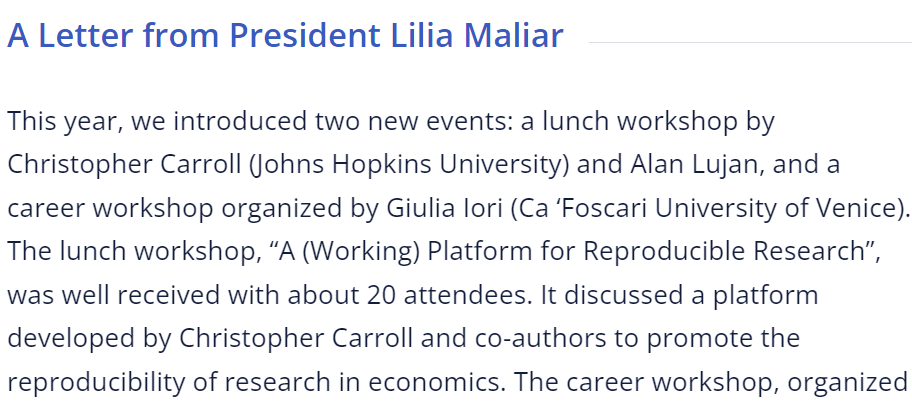
\includegraphics[width=0.7\linewidth]{files/sce_letter-993ec031415bd0f59891923fd6d8184d.png}
\caption*{An excerpt from A Letter from the Society for Computational Economics President Lilia Maliar describes the REMARK project presentation at the 30th International Conference for Computing in Economics and Finance. This screenshot was taken from \href{https://comp-econ.com/}{the SCE website}.}
\end{figure}

The presentation consisted of introducing the REMARK standard, demonstrating the capabilities of REMARKs through a live interactive presentation, and discussing the benefits of reproducibility in economics.

After the presentation, we received feedback from researchers who were very interested in the REMARK standard and were eager to introduce their students to the newly developed tools. We would love to take this presentation and workshop on the road and introduce REMARKs to the next generation of economists.

\begin{figure}[!htbp]
\centering
\caption*{A recap of our presentation at CEF 2024 and a discussion of REMARKs with the \href{https://opensource.science/}{OpenSource.Science} Economics interest group.}
\end{figure}

\subsection{Technical Milestones}

% Discuss any specific technical milestones achieved, such as code releases, documentation updates, or bug fixes. Quantify accomplishments with metrics where possible (e.g., user growth, code contributions).

A significant milestone of this project was the expansion of MyST compatibility with the $\LaTeX$ syntax. Many existing REMARKs are written in $\LaTeX$, and it is critical to ensure backward compatibility and the ability to refresh existing REMARKs with new MyST capabilities, including rich cross-references, hover previews, and (most importantly) integrated computation. Although we have not yet reached the goal of complete backward compatibility, we have made considerable progress in this area. We welcome contributions from the open source community to help us reach this goal.

Second, we started work on a \texttt{remark} command-line-interface tool that can be used to generate REMARK templates and check them against the REMARK standard. This tool also includes functionalities for building environments and running reproducibility scripts.

Third, we have continued to expand the catalog of existing REMARKs, including several new REMARKs of student projects and active research projects both within and outside \href{https://econ-ark.org/}{Econ-ARK}.

\subsection{Challenges and Solutions}

% Share any challenges encountered during the project and how you addressed them.

The project has gone quite smoothly, thanks to the deep expertise and strongly aligned goals of the REMARK project with the Myst project. The principal challenge is simply that making use of the new technologies requires an investment of time, which is the scarcest resource among busy scholars.

\section{Outcomes and Impact}

\subsection{Project Impact}

% Describe the positive impact of the project on the Hopkins community, the open source software ecosystem, or any other relevant groups. Use concrete examples and data to support your claims where possible.

The overarching objective of REMARK is to improve the reliability and trustworthiness of scientific findings within fields heavily reliant on computational methods. By promoting the use of standardized tools and workflows, the REMARK project aims to make computational research in economics and social sciences more transparent and reproducible.

REMARK encourages the adoption of best practices in software development, documentation, and manuscript preparation within the economics community, which has traditionally lagged behind other fields in which computational results are first-class scholarly contributions. Our goal is to facilitate knowledge sharing and collaboration, reduce duplication efforts, and accelerate the dissemination of knowledge within the field.

\subsection{Community Engagement}

% Did you actively engage with the open source community through contributions, conferences, or workshops? Share details and metrics of participation.

Our team primarily engaged with the main developers of the \href{https://github.com/jupyter-book/mystmd}{MyST} project through consultants at \href{https://curvenote.com/}{Curvenote}. We set up a weekly meeting where we discussed our needs for the REMARK project and suggestions for improving the MyST project itself. The team at MyST/Curvenote is deeply experienced and is closely connected with the open science and publishing communities.

Additionally, we advocated for the use of reproducibility standards at the 30th International Conference for Computing in Economics and Finance and at the \href{https://opensource.science/}{OpenSource.Science} Economics interest group. We met with many students and researchers interested in open source software for reproducible research and advocated for the adoption of REMARKs as a standard for reproducible research in Economics.

\subsection{Sustainability and Future Plans}

% Explain how the project will be sustained beyond the grant period. Are there plans for future development, funding, or community support? Is there potential for further impact?

\subsubsection{Renaming the project}

The need for the REMARK standard arose from our desire to make research conducted as part of the \href{https://econ-ark.org}{Econ-ARK} project easily reproducible and shareable -- an origin that is transparently signaled by the fact that the acronym is derived from ``R[eplications]/[eproductions] and Explorations Made using ARK.''

Now that the REMARK standard is completely independent of the Econ-ARK toolkit, this name is inappropriate, because it will mislead people into thinking they must be using the Econ-ARK toolkit if they want to create a reproducible software object using these tools.

To address this issue, we have discussed internally the need to rename the project, with the current leading candidate name \textbf{``SCI-PASS''}, which stands for ``Scholarly Communication Infrastructure for Publishing and Archiving Scientific Software.'' This name change captures our current ambition of establishing a universal and inclusive standard for reproducible scientific software.

Renaming REMARK is not a cosmetic change; it is a signal of our ambition to build a robust standard for reproducible computational research of any kind. The near-term evolution of the project will be guided by our interactions with the editor of the prospective journal mentioned above, as we develop it into submission standard for scientific and technical journal articles. We will continue actively engaging with the scientific community to improve and promote the standard and foster collaboration, including establishing communication channels with existing journal editors, journal data editors, and others who already have expertise and wisdom to offer on these topics. consider ``SCI-PASS'' to be short for ``scientific passport,'' a term that encapsulates the idea of portability and exchangeability of research outputs.

\begin{framed}
\textbf{Important}\\
\textbf{SCI-PASS} stands for:

\begin{enumerate}
\item \textit{Scholarly Communication Infrastructure for Publishing and Archiving Scientific Software} - a new name for the REMARK project to better reflect its scope and potential for broader adoption.
\item \textit{Scientific Passport} - enables scientific software to be portable across different environments.
\end{enumerate}
\end{framed}

\subsubsection{Adapting to Evolving Research Practices}

To succeed, the REMARK/SCI-PASS project must embrace modern publishing technologies. As we recognized the limitations of $\LaTeX$, this grant helped us integrate modern scientific publishing tools like \href{https://jupyter.org}{Jupyter Notebooks} and MyST Markdown. This shift toward the Jupyter ecosystem is intended to enhance user-friendliness, interactivity, and accessibility for researchers. In the long-term, we aim to further integrate with open science infrastructure, such as established open science publishing platforms for peer-review and publishing like \href{https://theoj.org/}{Open Journals} and \href{https://joss.theoj.org/}{The Journal of Open Source Software}.

While most existing REMARKs are built using \texttt{python}, we are committed to expanding language support to accommodate the diverse set of tools used in computational research. This expansion aims to broaden the project's reach and applicability across disciplines. Moreover, the project's long-term sustainability depends on active community engagement, which includes collaborating with journal and data editors, organizing workshops and tutorials, and establishing an independent board of advisors with expertise in computational science, library science, and relevant research domains. By embracing these adaptations, the REMARK/SCI-PASS project aims to evolve into a robust and sustainable standard for reproducible research, aligning with evolving practices and solidifying its place within the future of open science.

\subsubsection{Taking REMARK/SCI-PASS on the road}

This grant allowed us to host a workshop at the 30th International Conference for Computing in Economics and Finance in Singapore, where we discussed open science, reproducibility, and the REMARK standard. The experience and feedback we gathered were invaluable, and we are eager to take the project on the road to more conferences and events. Below, we describe a few of the ways in which we plan to advocate for open science and reproducibility:

\begin{enumerate}
\item \textbf{Replication Competitions} - Competitions where researchers are challenged to replicate the results of notable papers, which will provide a practical demonstration of the REMARK standard and incentivize adoption.
\item \textbf{Tutorials and Workshops} - Target students and researchers to provide hands-on experience using our tools, demonstrating how to create reproducible research outputs and highlighting the advantages of open science.
\item \textbf{Talks} - Engage with journal editors and data editors to seek feedback and collaboration to understand better how our project can streamline the review process, ensure reproducibility, and enhance the credibility of published research.
\end{enumerate}

% ## Lessons Learned

% Share key takeaways and insights gained from the project.

% ## Attachments

% Include relevant documents such as screenshots, code samples, documentation updates, or presentations.

\section{Financial Information}

\subsection{Grant Expenditures}

% Provide a detailed breakdown of how the grant funds were used. This should be consistent with the approved budget in the grant proposal.

\begin{framed}
\textbf{Attention}\\
Please see the attached Financial Report for a detailed breakdown of how the grant funds were used.
\end{framed}

The majority of the funds were used to contract with Curvenote to integrate the MyST tools into the REMARK project. We also supported the work of three Johns Hopkins University PhD students over the summer of 2024 to produce REMARKs on their ongoing research projects. Finally, we hosted a workshop at the 30th International Conference for Computing in Economics and Finance in Singapore and used the remaining funds for travel and lodging.

% ## Budget Variance

% Explain any significant deviations from the original budget.

\section*{Acknowledgments}
This project was funded by the \href{https://jhu.edu}{Johns Hopkins University} \href{https://ospo.library.jhu.edu/}{Open Source Programs Office}, and the \href{https://sloan.org}{Alfred P. Sloan Foundation}.



\end{document}
